\newgeometry{left=3cm,right=3cm,bottom=3cm,top=3cm}
\thispagestyle{empty}
\begin{center}

\includegraphics[height=5cm]{Figure/LOGO_UNISI.pdf}

\large{ \sc Dipartimento di ingegneria dell'informazione e scienze matematiche}
\vspace{0.5cm
\large Computer and Automation Engineering}\\
\vspace{0.5cm}
\large {\sc Robotics and Automation}
\vspace{1cm}
 
\vspace{\stretch{.8}}

%\textbf{\scshape{\LARGE{Handwritten classification of MNIST dataset\\with TensorFlow\\}}}
\textbf{\scshape{\LARGE{Closed loop approach to human-robot handshake\\}}}

\end{center}
\vspace{\stretch{1}}

\noindent\begin{minipage}[b]{0.47\textwidth}
\begin{flushleft} 
\large
\emph{Supervisor:}\\
\textit{Chiar.ssimo} \textbf{D. Prattichizzo}  
\emph{Co-supervisor:}\\
\textit{?} \textbf{M. Malvezzi}\\
\textit{?} \textbf{E. Knoop}

\end{flushleft}
\end{minipage}
\hfill
\begin{minipage}[b]{0.47\textwidth}\raggedleft
 \large
\emph{Student:}\\
\textbf{Francesco Vigni}\\


\end{minipage}

%\begin{minipage}{0.5\textwidth}
%\begin{flushright} \large
%\emph{Tesi di laurea di:} \\
%\textbf{Francesco Vigni}
%\end{flushright}
%\end{minipage}
%
%\begin{minipage}[t]{0.47\textwidth}
%{\large{\bf Relatore:\\
%Prof. NOME RELATORE}}
%\vspace{5mm}\\
%{\large{\bf Correlatore:\\
%Prof. NOME CORRELATORE\\
%Prof. NOME CORRELATORE}}\\
%%\vspace{5mm}\\
%%{\large{\bf Relatore:\\
%%Chiar.mo Prof.\\
%%NOME CORRELATORE}}
%\end{minipage}
%\hfill
%
%\begin{minipage}[t]{0.47\textwidth}\raggedleft
%{\large{\bf Candidato:\\
%NOME LAUREANDO}}
%\end{minipage}


%\noindent RELATORI:\\
%Prof. Gigi Riva\\
%Prof. alskdj
%\begin{flushright}
%TESI DI LAUREA DI:\\
%kjsad aslkjd 

%\end{flushright}
%\vspace{\stretch{1}}
%\vfill
\begin{center}
\hrule
%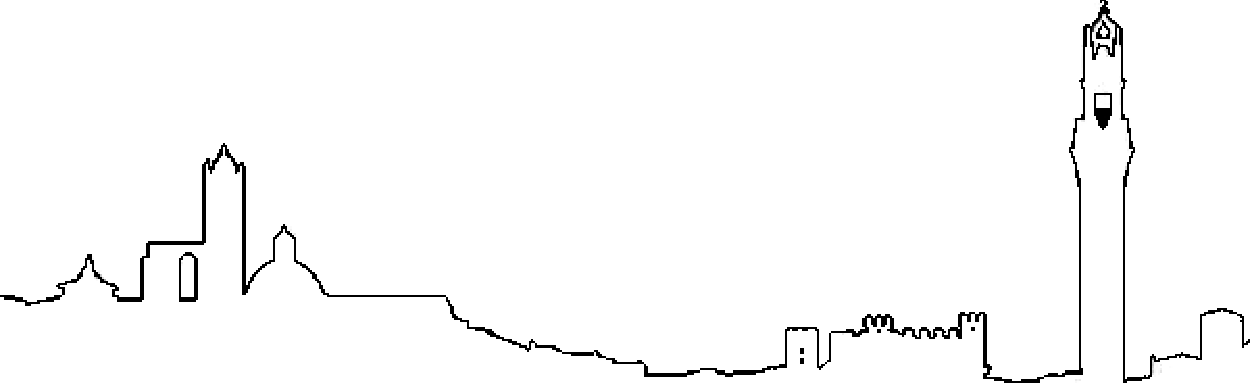
\includegraphics[width=\columnwidth]{figure/skyline1}
\vspace{0.5cm}
\large{A.A. 2017-2018}
\end{center}
\restoregeometry


